\section{\ttt{3D} classification and Refinement}

 \begin{figure}[H]
  \centering
  \captionsetup{width=.8\linewidth} 
  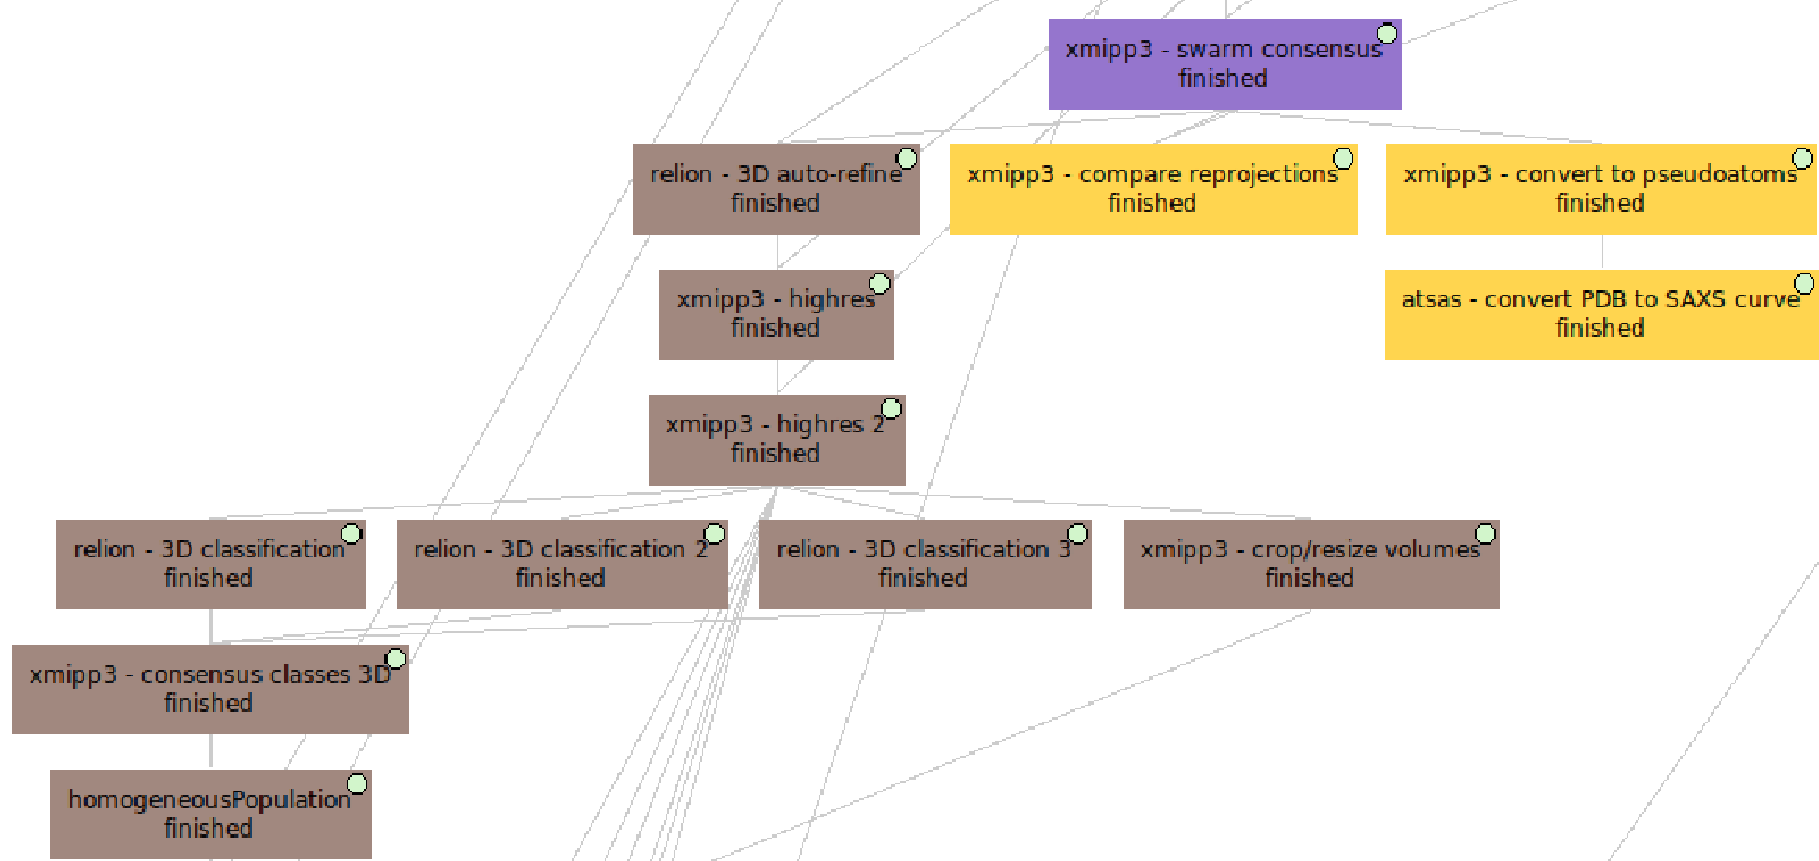
\includegraphics[width=1\textwidth]
  {{images/workflow_6.pdf}}
  \caption{Refinement and \ttt{3D} classification (Brown color).}
  \label{fig:workflow_6}
  \end{figure}

\ttt{3D} classification and Refinement are the two last overlapping steps in image processing. They consume the most time and resources with the aim of obtaining a \ttt{3D} map at the highest possible resolution. This is only feasible if data are homogeneous enough, $i.e.$, if data represent a unique conformation of the specimen.\\

\subsection*{Refinement of the initial map}
Before starting with the \ttt{3D} classification properly, three consecutive steps of refinement will be performed with our initial map. The first approach to get a high resolution map in a fully automated manner was performed with the algorithm $Relion$ \ttt{auto\_refine}, based on an empirical Bayesian approach. This procedure employs the so-called gold-standard Fourier Shell Correlation (FSC) to estimate the resolution. Combined with a novel procedure to estimate the accuracy of the angular assignments, the algorithm converges. We have implemented it in the protocol \scommand{relion- \ttt{3D} auto-refine} (\ffigure{fig:initial_vol_1}). In the \ttt{Input} tap of this protocol form we include the subset of homogeneous particles  selected previously. The initial volume will be included in the \ttt{Reference 3D map} tap, as well as a \ttt{Initial low pass-filter (A)} of 60.0. This tap gives you the possibility of using \ttt{Reference mask (optional)} and, in some cases, $e.g.$ non-empty icosahedral viruses, a \ttt{Second reference mask (optional)}.

\begin{figure}[H]
  \centering
  \captionsetup{width=.8\linewidth} 
  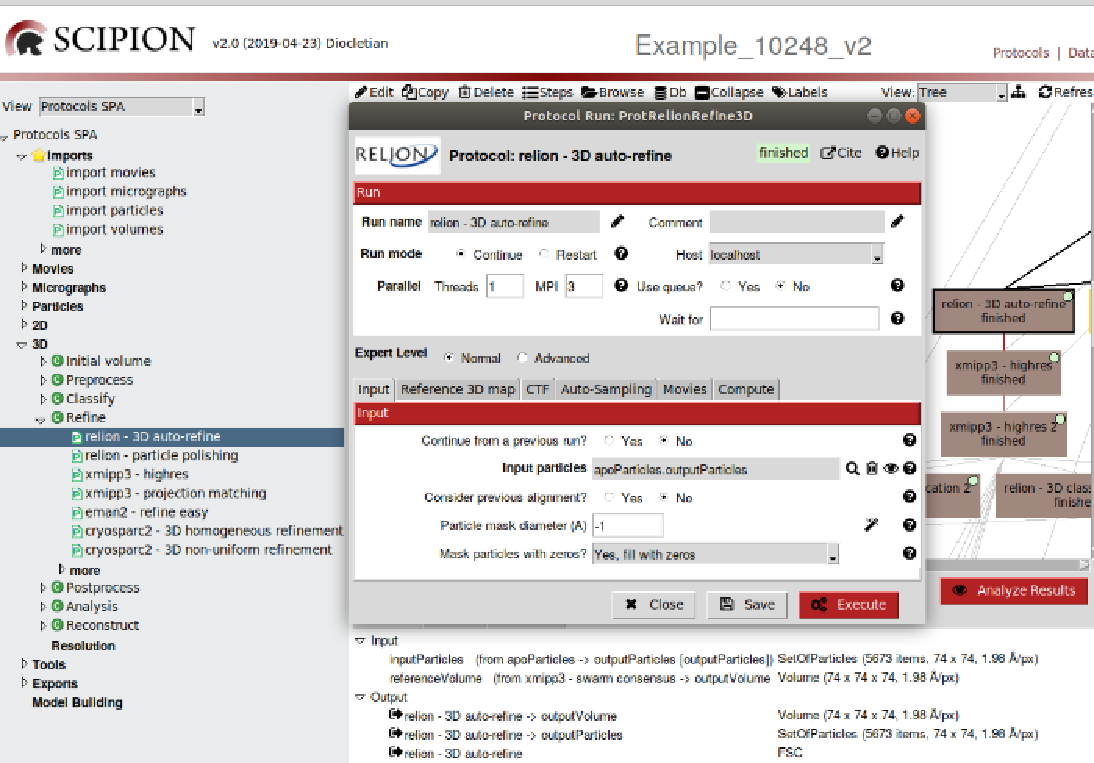
\includegraphics[width=0.95\textwidth]
  {{images/relion_3D_auto_refine_1.pdf}}
  \caption{Completing the params of the protocol \scommand{relion- \ttt{3D} auto-refine}.}
  \label{fig:relion_3D_auto_refine_1}
  \end{figure}

There are three questions in the tab \ttt{CTF}: 
\begin{itemize}
 \item \ttt{Do CTF correction?}, set to \ttt{Yes} to perform full phase + amplitude CTF correction.
 \item \ttt{Has reference been CTF-corrected?}, set to \ttt{No} because the Fourier transforms of the reference projections are not multiplied by the \ttt{CTF} in the first iteration. 
 \item \ttt{Do manual grouping ctfs?}, set to \ttt{No} because we have enough number of particles that we do not need to group them.
\end{itemize}

The \ttt{Angular sampling interval (deg)} option in the tab \ttt{Auto-Sampling} will be used only in the first few iterations. Later, the algorithm will automatically increase its value until convergence. For symmetries lower than octahedral or icosahedral we use the default values of \ttt{Angular sampling interval (deg)} and \ttt{Local search from auto-sampling (deg)}.\\

\ttt{Movies} tab allows to align movie-particles of each frame and execute later a protocol of particle polishing.\\

After executing 7 iterations, a refined map of 5.05 \AA\ of final resolution was obtained as output, with the same size and sampling rate that we had in the inputs. Press \scommand{Analyze Results} and visualize any iteration or the last one by default. Concerning particles, their angular assignment and the \ttt{\*\_optimiser.star file}, with general information about the refinement process, can be shown. Different volumes can be \ttt{2D} or \ttt{3D} visualized, such as each half map, both, or the final one. \ttt{SSRN} and resolution \ttt{FSC} plots are also available.\\

The next two following steps of refinement have been performed with the $Xmipp$ algorithm \ttt{highres} \citep{sorzano2018new} that we have implemented in the protocol \scommand{xmipp3-highres} (\ffigure{fig:xmipp_highres_1}). This method computes a weight for each particle and performs both global and local alignment. Iterations can be performed one by one, removing particles that worse fit the map from one iteration to the next one. This \ttt{3D} refinement protocol uses as input the refined map obtained from $Relion$ \ttt{auto\_refine} and the same set of particles used by this algorithm. The \ttt{Symmetry group} has been also included in the \ttt{Input} tap. In the \ttt{Angular assignment} tap we choose \ttt{Global} as \ttt{Image alignment} and 1 \ttt{Number of iterations} with 4 \AA\ as \ttt{Max. Target Resolution}.

\begin{figure}[H]
  \centering
  \captionsetup{width=.8\linewidth} 
  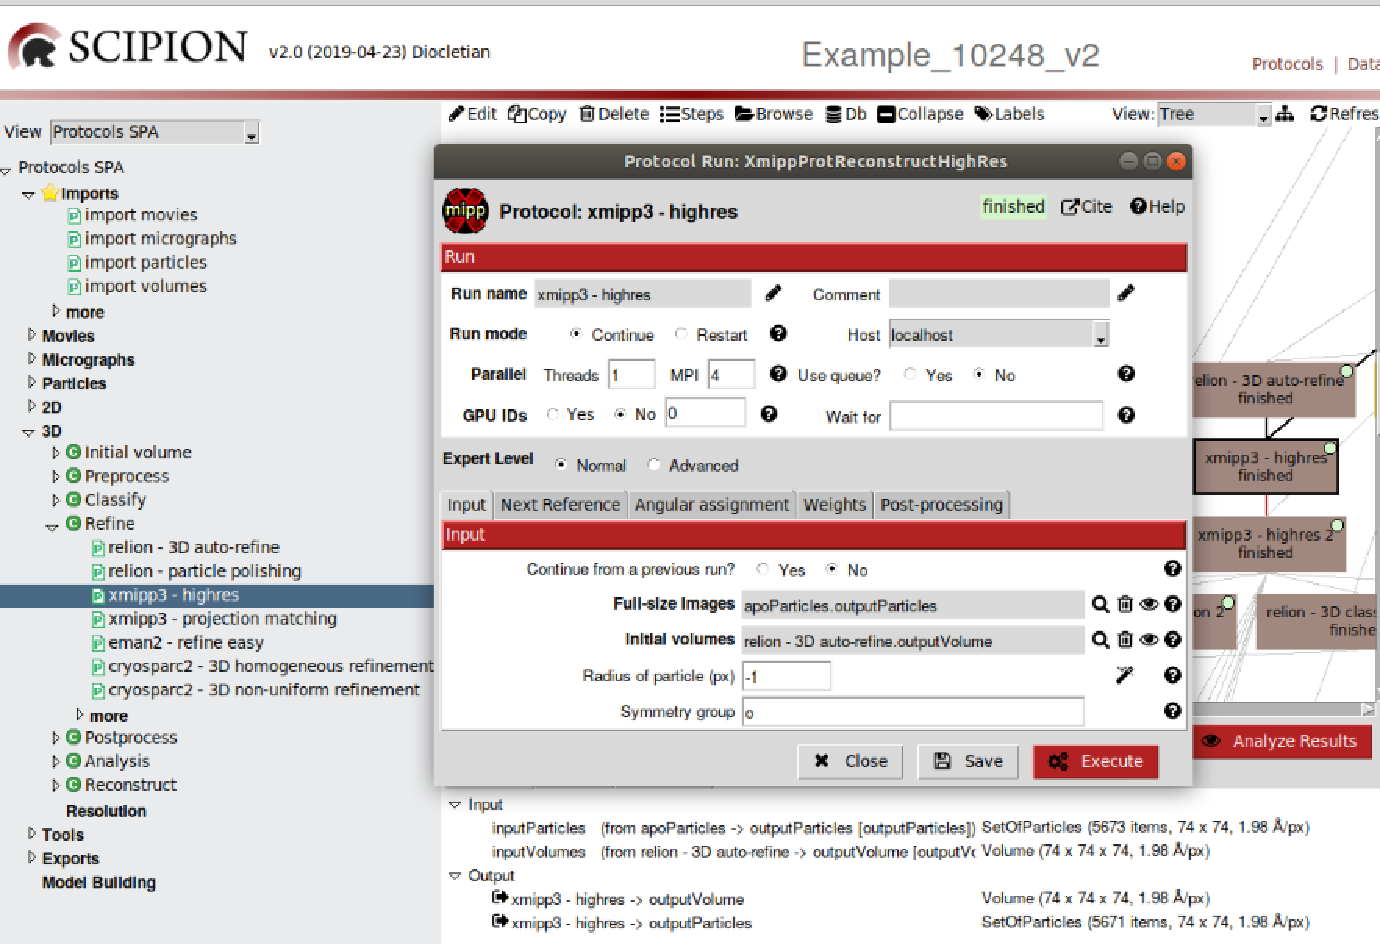
\includegraphics[width=0.95\textwidth]
  {{images/xmipp_highres_1.pdf}}
  \caption{Filling in the params of the protocol \scommand{xmipp3-highres}.}
  \label{fig:xmipp_highres_1}
  \end{figure}

This protocol also generates one map as output with the initial size and sampling rate. Press \scommand{Analyze Results} to check the results of the iteration 1. Particles and map can also visualized. 2 particles have been rejected.\\

The second time that we execute the protocol \scommand{xmipp3-highres} we select the map obtained in the previous step and the same set of particles as input. In the tap \ttt{Angular assignment} we replace \ttt{Global} by \ttt{Local} in the \ttt{Image alignment} param. The rest of the params remain unchanged since we have selected \ttt{Yes} in the param \ttt{Continue from a previous run?} of tap \ttt{Input}. In this case, another map has been generated as output with the same size and sampling rate. 6 particles have been discarded this time.\\

\subsection*{3D classification}
To continue with the refinement process and to obtain a better resolution, we start executing three independent times the same algorithm of $Relion$ \ttt{3D classification} that we have implemented in the protocol \scommand{relion-3D classification} (\ffigure{fig:relion_3Dclassification}). In the tap \ttt{Input} we include the particles derived from executing the previous protocol \scommand{xmipp3-highres}. The map derived from this protocol will be the \ttt{Input volume(s)} in the tap \ttt{Reference 3D map}. The optimization params appear in the tap \ttt{Optimization}: 3 \ttt{Number of classes} and 25 \ttt{Number of iterations}. As \ttt{Regularisation parameter T} values as 3-4 are common for \ttt{3D} classificacion.

\begin{figure}[H]
  \centering
  \captionsetup{width=.8\linewidth} 
  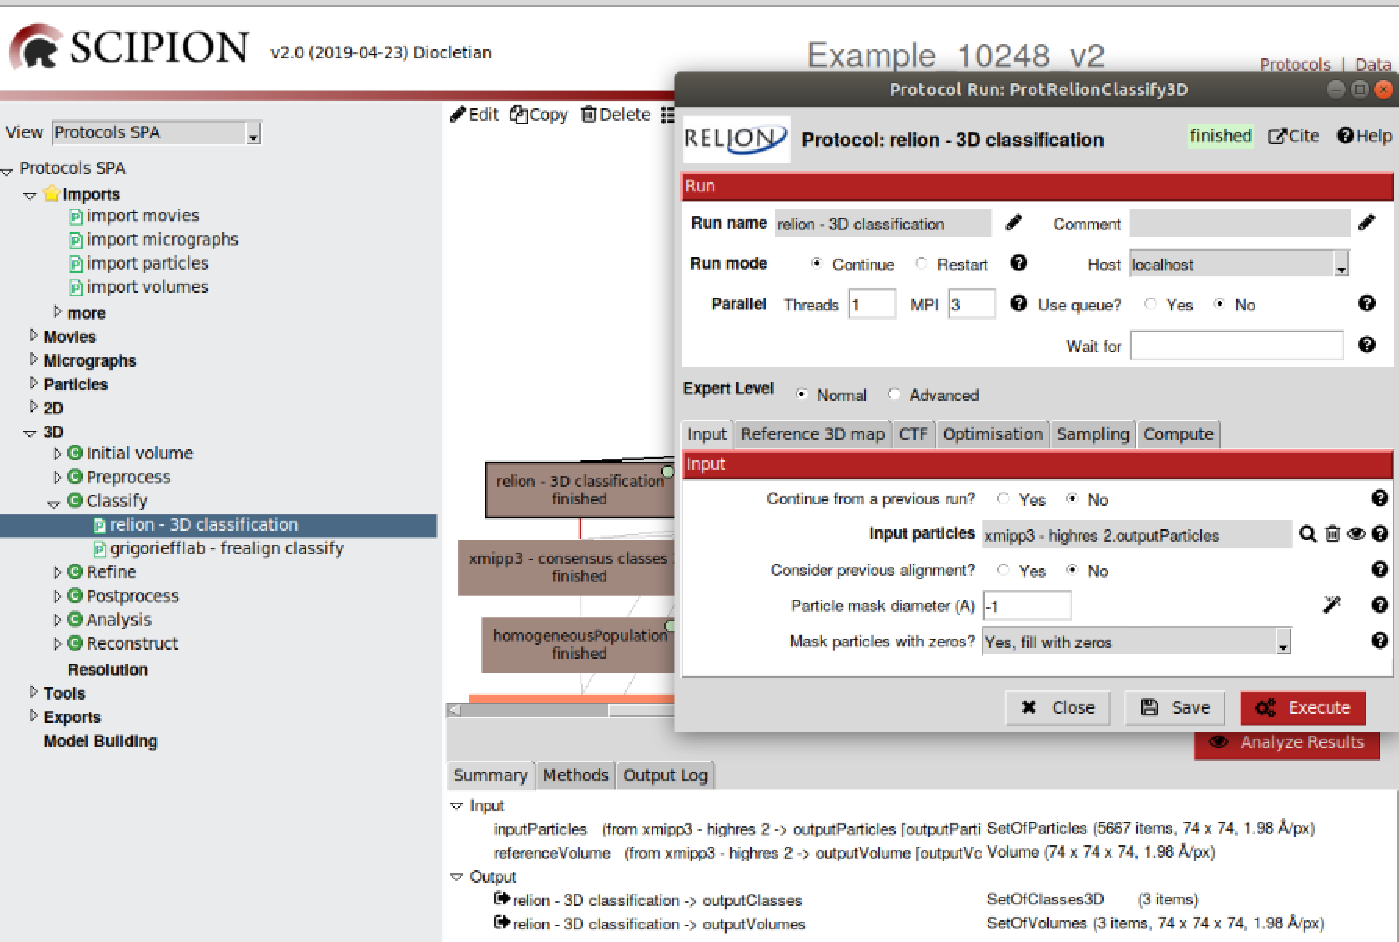
\includegraphics[width=0.95\textwidth]
  {{images/relion_3Dclassification.pdf}}
  \caption{Completing the params of the protocol \scommand{relion-3D classification}.}
  \label{fig:relion_3Dclassification}
  \end{figure}
  
The output of each one of these three \scommand{relion-3D classification} protocols are 3 maps with the initial size and sampling rate, reconstructed from different groups of reclassified particles. By pressing \scommand{Analyze Results} and \ttt{Particles/ Show classification in Scipion}, a table will be opened showing the projection representative of each map and the number of particles contributing to its reconstruction:
\begin{itemize}
 \item 4,713, 886 and 68 in the first classification.
 \item 2,854, 2,739 and 74 in the second one.
 \item 4,964, 583 and 120 in the last one.
\end{itemize}

The results of the first and third \ttt{3D} classifications are similar because in both cases the first class contains most of the particles. However, in the second classification the first two classes are quite similar regarding the number of particles. In order to have a consensus of these three results, we execute the protocol \scommand{xmipp3-consensus classes 3D} that compares several sets of \ttt{3D} classes and return the intersection of the input classes (\ffigure{fig:consensus_classes}).

\begin{figure}[H]
  \centering
  \captionsetup{width=.8\linewidth} 
  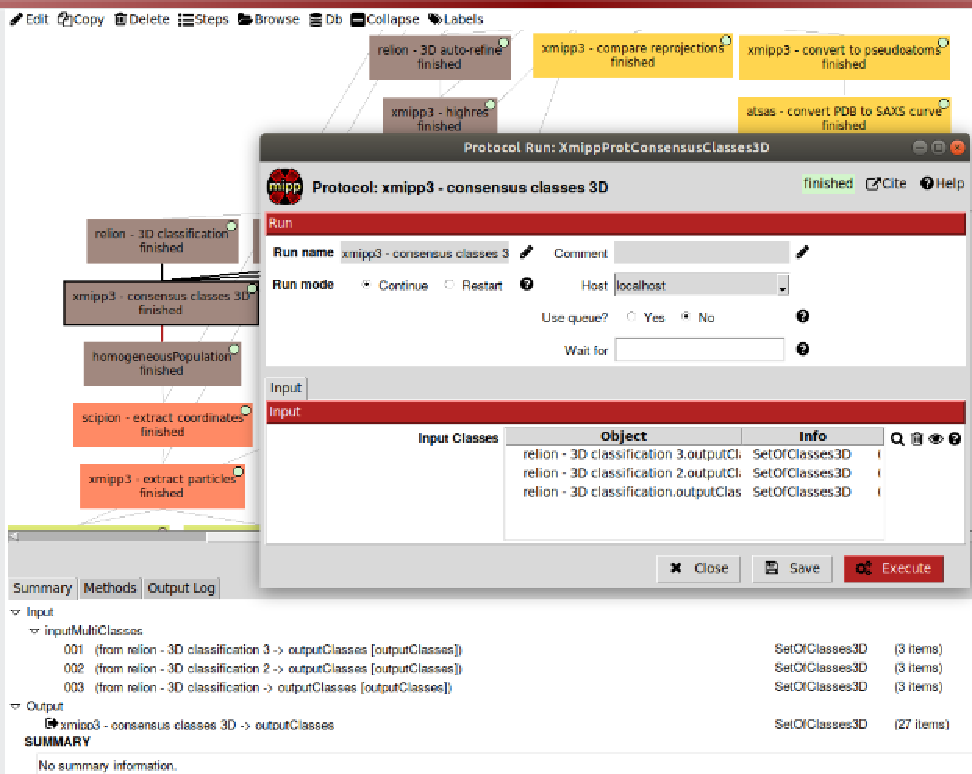
\includegraphics[width=0.95\textwidth]
  {{images/consensus_classes.pdf}}
  \caption{Filling in the params of the protocol \scommand{xmipp3-consensus classes 3D}.}
  \label{fig:consensus_classes}
  \end{figure}
  
By pressing \scommand{Analysis Results} you can visualize the 27 intersection \ttt{3D} classes with the number of particles assigned to each one. Two of these classes derive from about 2,000 particles (aprox. 75\% of total particles), 4 classes from 199-466 particles, 8 classes from 11-81 particles, and the other 13 classes from less than 10 particles.\\

 \begin{figure}[H]
  \centering
  \captionsetup{width=.8\linewidth} 
  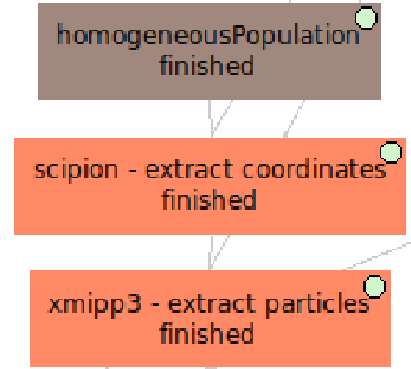
\includegraphics[width=0.30\textwidth]
  {{images/workflow_7.pdf}}
  \caption{Extraction of re-classified particles (Orange color).}
  \label{fig:workflow_7}
  \end{figure}
  
From this global population of reclassified particles (in brown in \ffigure{fig:workflow_7}) we are going to extract again particle coordinates from the CTF-corrected micrographs, using the protocol \scommand{xmipp3-extract coordinates} (\ffigure{fig:extract_coordinates}). This protocol allows to re-extract coordinates from particles with their original dimensions and visualize those particles in their locations on micrographs. The homogeneous population of particles previously obtained and the CTF consensus micrographs are the protocol input params.

\begin{figure}[H]
  \centering
  \captionsetup{width=.8\linewidth} 
  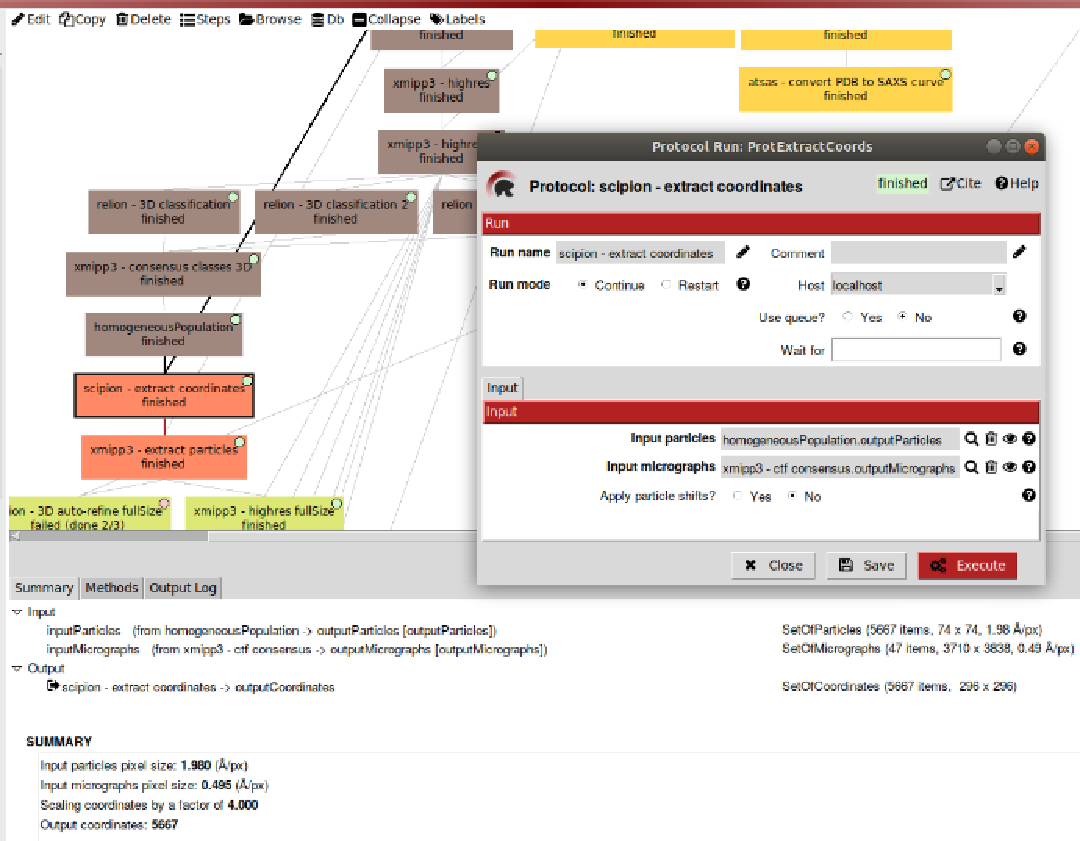
\includegraphics[width=0.95\textwidth]
  {{images/extract_coordinates.pdf}}
  \caption{Completing the params of the protocol \scommand{xmipp3-extract coordinates}.}
  \label{fig:extract_coordinates}
  \end{figure}

As output, \scommand{xmipp3-extract coordinates} generates the  5,667 particle coordinates scaled by a factor of 4.0. Press \scommand{Analyze Results} and observe the particles in each micrograph. These particles will be extracted with the above used protocol \scommand{xmipp3-extract particles} (\ffigure{fig:extract_particles_2}). The particle coordinates previously extracted and CTF-consensus micrographs will be inputs of the protocol, as well as the \ttt{Downsampling factor} of 1.0 and the \ttt{Particle box size (px)} of 450.

\begin{figure}[H]
  \centering
  \captionsetup{width=.8\linewidth} 
  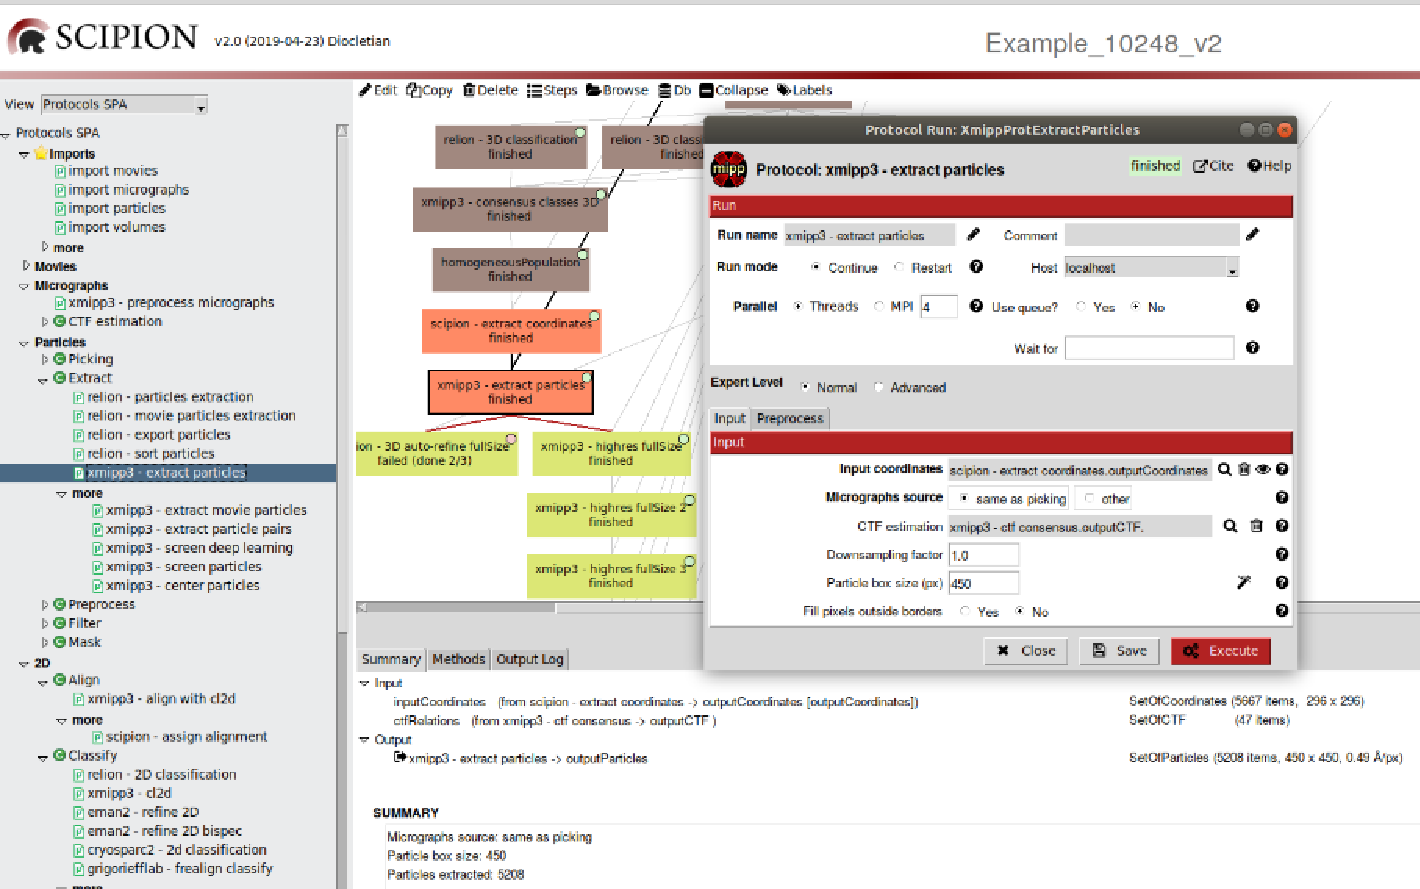
\includegraphics[width=0.95\textwidth]
  {{images/extract_particles_2.pdf}}
  \caption{Filling in the params of the protocol \scommand{xmipp3-extract particles}.}
  \label{fig:extract_particles_2}
  \end{figure}

The output of the protocol includes 5,208 particles (459 less than in the input) with the selected size and the starting sampling rate. Press \ttt{Analyze Results} to observe the table with the new set of particles.  

\subsection*{Final refinement iterations with $Xmipp$ \ttt{highres}}
 \begin{figure}[H]
  \centering
  \captionsetup{width=.8\linewidth} 
  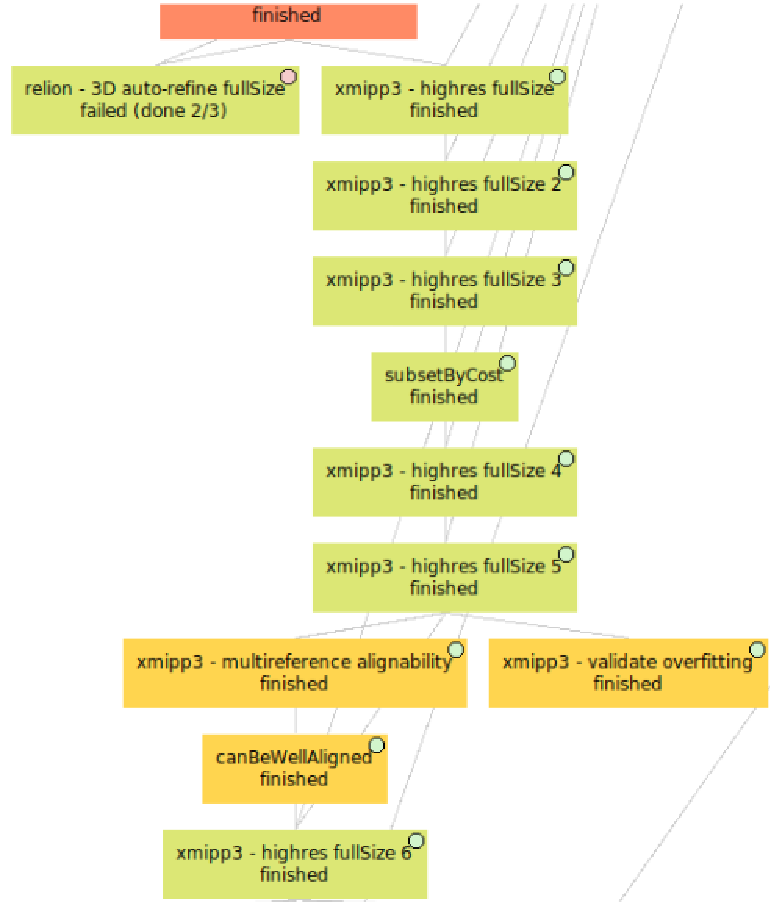
\includegraphics[width=0.7\textwidth]
  {{images/workflow_8.pdf}}
  \caption{Map final refinement (Light green color).}
  \label{fig:workflow_8}
  \end{figure}
  
From now ahead several steps of refinement will be accomplished using the above mentioned protocol \scommand{xmipp3-highres}. The input of the first round of refinement includes the particles extracted with the previous protocol and the volume generated by the same algorithm before performing the \ttt{3D} classification step (\ffigure{fig:highres_fullsize}). In the \ttt{Angular assignment} tap, we select \ttt{Global} for the \ttt{Image alignment} param, 1 as \ttt{Number of iterations} and 3 as \ttt{Max. Target Resolution}.

 \begin{figure}[H]
  \centering
  \captionsetup{width=.8\linewidth} 
  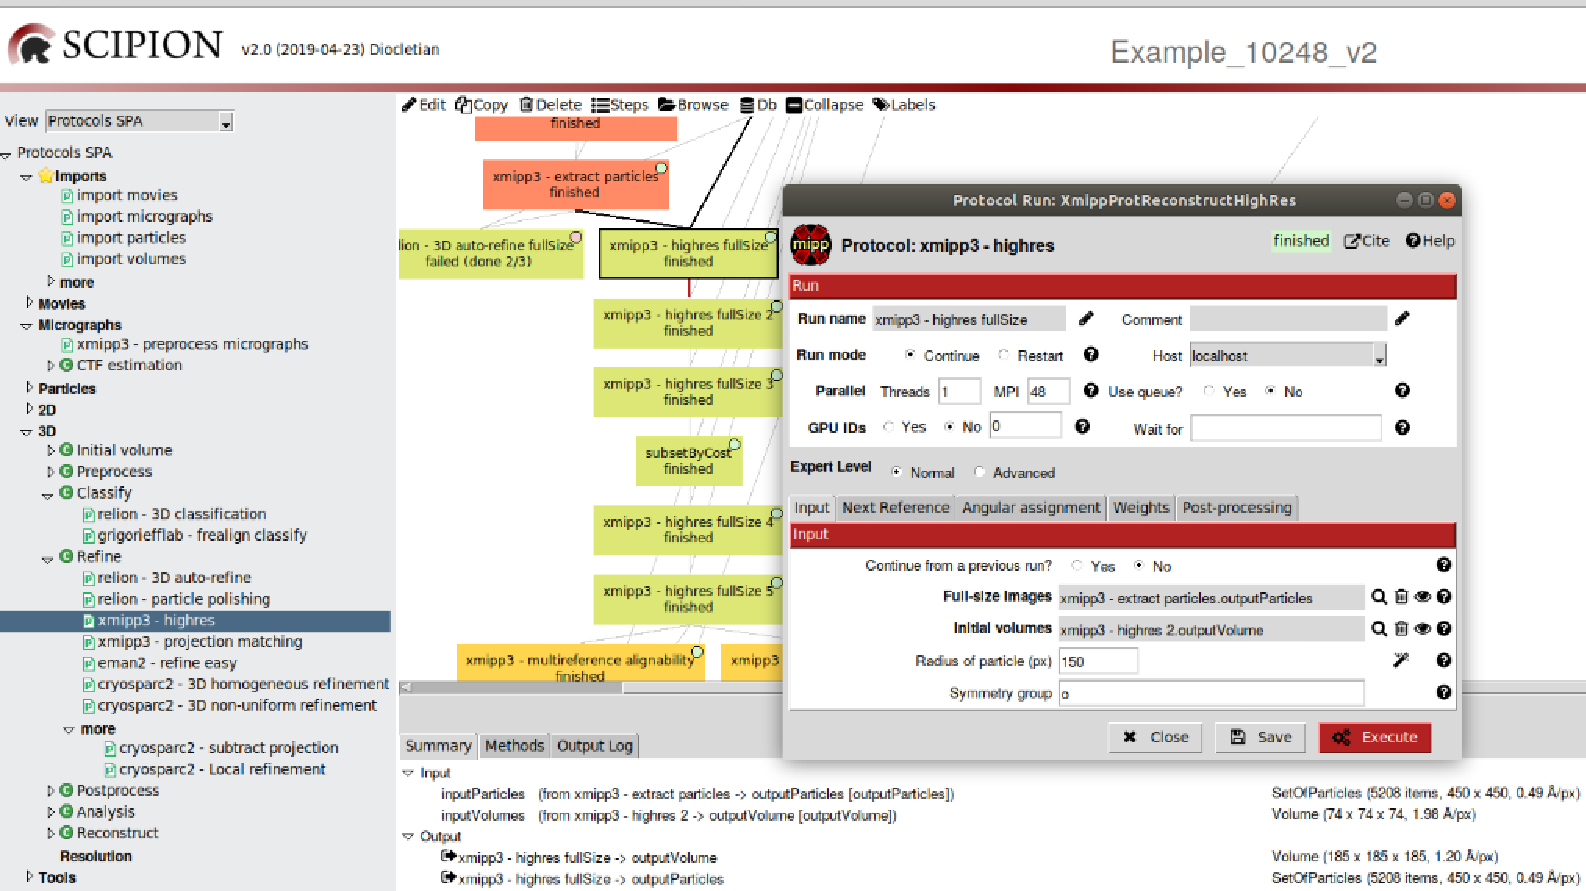
\includegraphics[width=0.95\textwidth]
  {{images/highres_fullsize.pdf}}
  \caption{$Xmipp$ \ttt{highres} map global refinement (Iteration 1).}
  \label{fig:highres_fullsize}
  \end{figure}
  
The output resampled volume generated can be seen by pressing \scommand{Analyze results}, as well as the particles from which it derives.\\

The second run of refinement continues from the previous one, as it is selected in the \ttt{Input} tap. The particles derived from the first round of refinement are included as input params. The same params have been selected in the \ttt{Angular assignment} tap (\ffigure{fig:highres_fullsize2}).

 \begin{figure}[H]
  \centering
  \captionsetup{width=.8\linewidth} 
  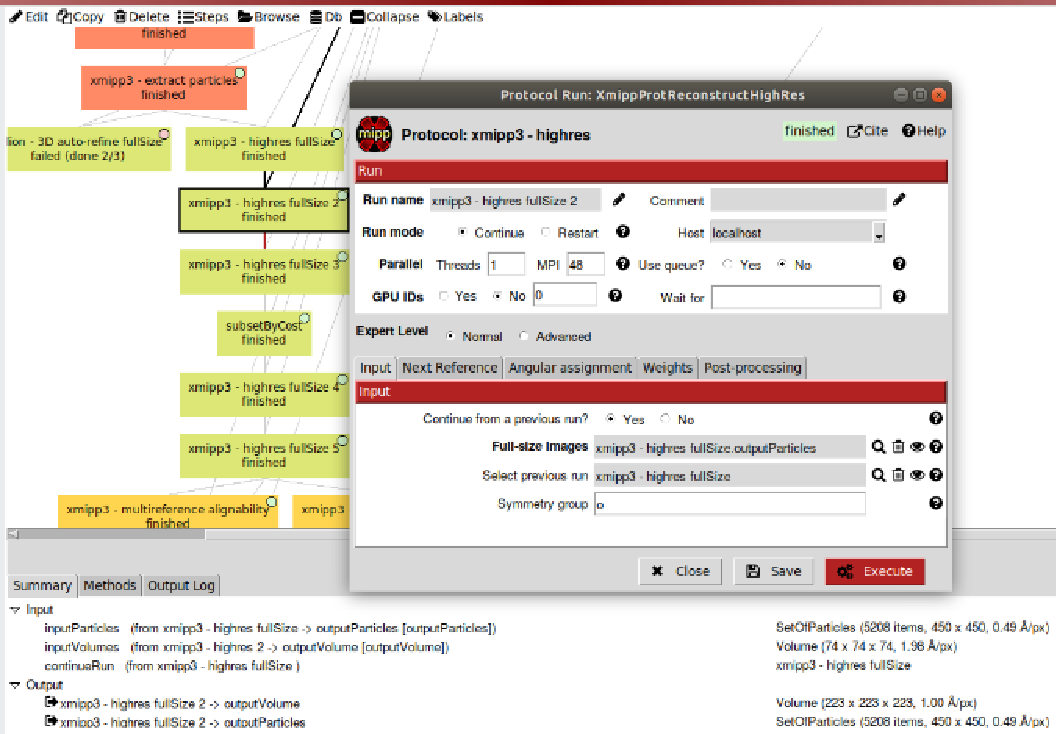
\includegraphics[width=0.95\textwidth]
  {{images/highres_fullsize2.pdf}}
  \caption{$Xmipp$ \ttt{highres} map global refinement (Iteration 2).}
  \label{fig:highres_fullsize2}
  \end{figure}

A new output resampled volume has been obtained that move from 1.20 \AA/px to 1.00 \AA/px).\\

Once we have finished the global refinement, we continue with the local refinement in the third round of refinement (\ffigure{fig:highres_fullsize3}). Again, we use the particles derived from the previous iteration. In this case, we select \ttt{Local} for the \ttt{Image alignment} param and 2.5 for the \ttt{Max. Target Resolution} of tap \ttt{Angular assignment}. \ttt{Shifts} and \ttt{angles} will be also optimized.

 \begin{figure}[H]
  \centering
  \captionsetup{width=.8\linewidth} 
  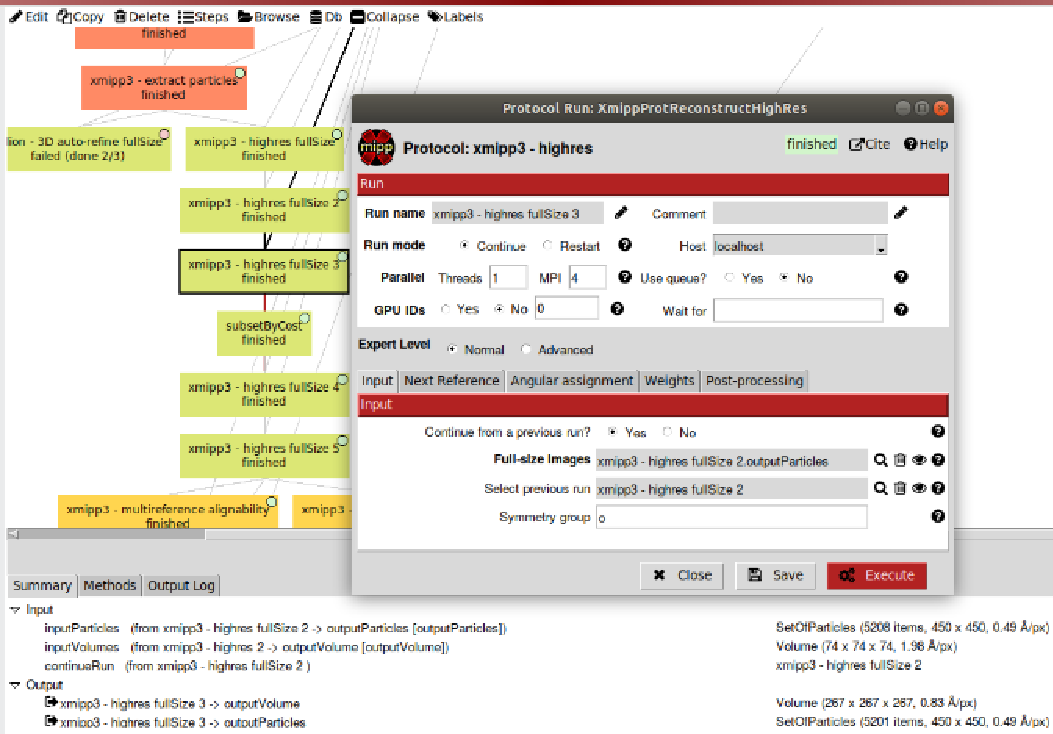
\includegraphics[width=0.95\textwidth]
  {{images/highres_fullsize3.pdf}}
  \caption{$Xmipp$ \ttt{highres} map local refinement (Iteration 3).}
  \label{fig:highres_fullsize3}
  \end{figure}

The output resampled volume obtained (0.83 \AA/px) derives from a set of particles slightly smaller (5,201). The table of particles can be also observed by pressing \scommand{Analyze results}. We can select particles according to the value of the \ttt{\_xmipp\_cost} param. Choosing values higher than 0.15, a total of 696 particles (13.4\%) of the input set has been removed. The remaining 4,505 particles will be used as inputs of the fourth round of refinement (\ffigure{fig:highres_fullsize4}). Params from \ttt{Angular assignment} tap will remain unchanged except the \ttt{Optimization} ones. In addition to \ttt{shifts} and \ttt{angles}, \ttt{scale} and \ttt{defocus} will be also optimized.

\begin{figure}[H]
  \centering
  \captionsetup{width=.8\linewidth} 
  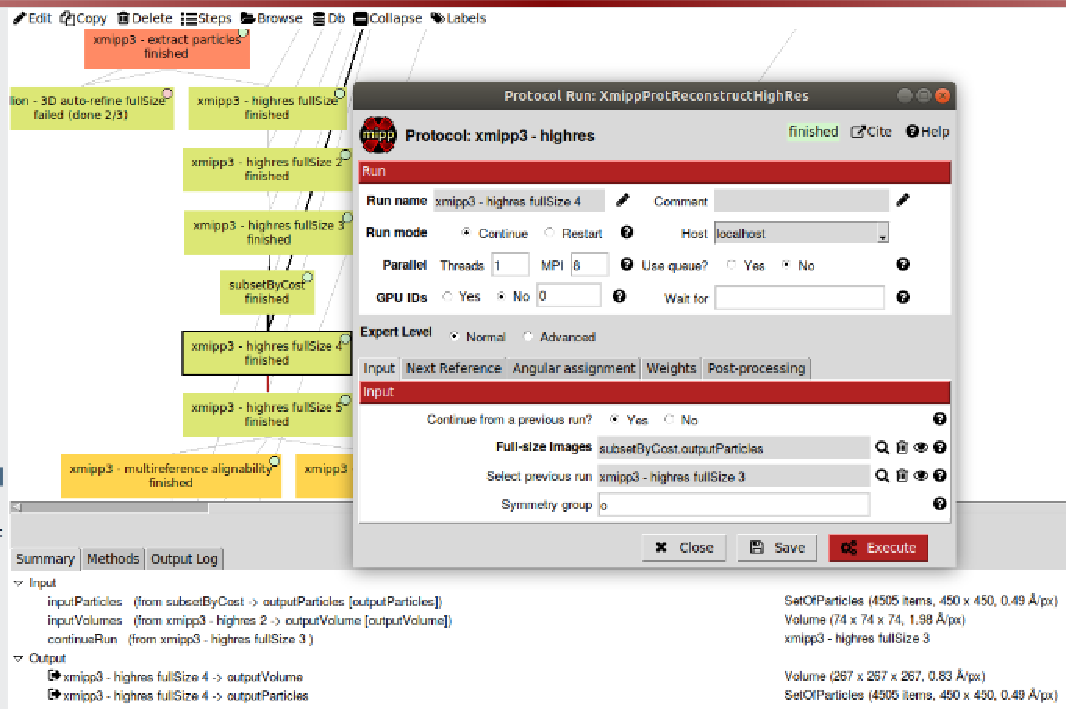
\includegraphics[width=0.95\textwidth]
  {{images/highres_fullsize4.pdf}}
  \caption{$Xmipp$ \ttt{highres} map local refinement (Iteration 4).}
  \label{fig:highres_fullsize4}
  \end{figure}
  
The new map, based on the last set of particles, appears in the output. These particles are included in the input of the fifth round of local refinement (\ffigure{fig:highres_fullsize5}). This time, we reduce the value of the \ttt{Max. Target Resolution} param to 2.25 and set to \ttt{Yes} all the \ttt{Optimization} params.

\begin{figure}[H]
  \centering
  \captionsetup{width=.8\linewidth} 
  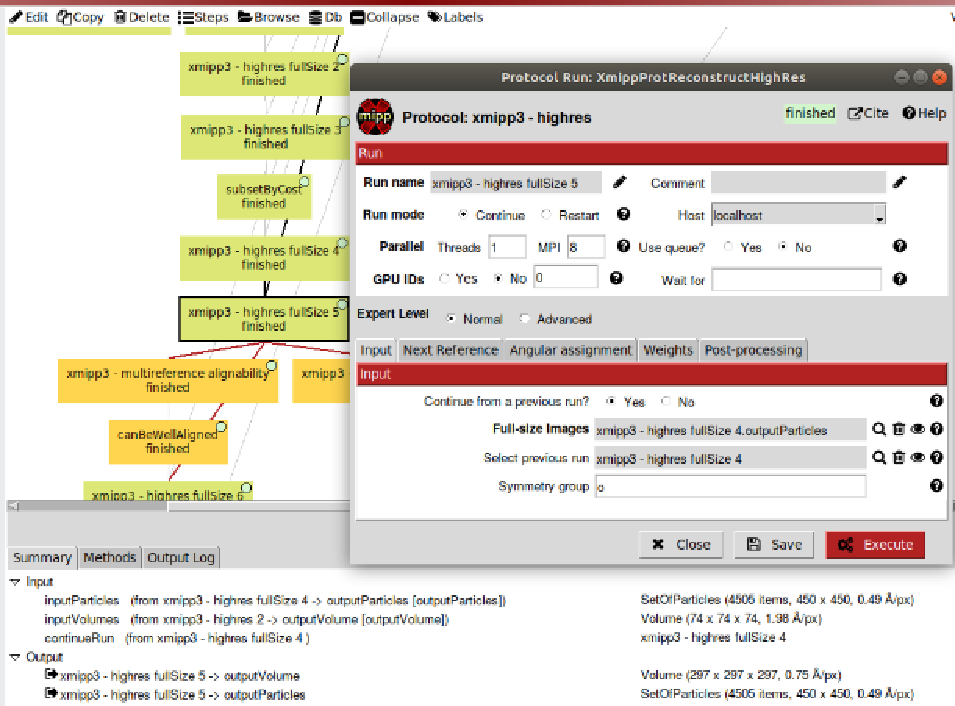
\includegraphics[width=0.95\textwidth]
  {{images/highres_fullsize5.pdf}}
  \caption{$Xmipp$ \ttt{highres} map local refinement (Iteration 5).}
  \label{fig:highres_fullsize5}
  \end{figure}
  
Before continuing with the sixth round of refinement we are going to assess the output resampled map (0.75\AA/px) regarding soft alignability and overfitting of particles and \ttt{3D} map. Two protocols are going to be independently executed: \scommand{xmipp3-multireference alignability} (\ffigure{fig:multireference_alignability}) and \scommand{xmipp3-validate overfitting} (\ffigure{fig:validate_overfitting}). The input of both protocols requires map and particles generated in the last refinement iteration. 

\begin{figure}[H]
  \centering
  \captionsetup{width=.8\linewidth} 
  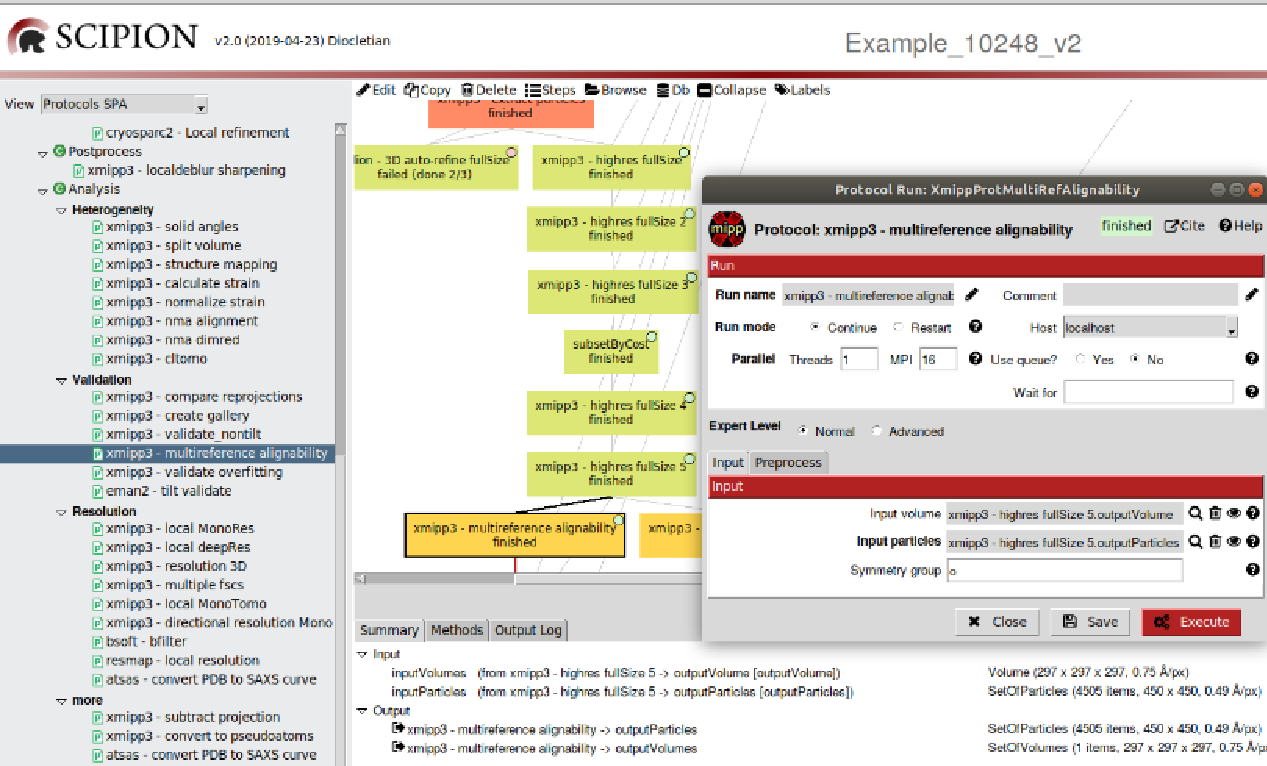
\includegraphics[width=0.95\textwidth]
  {{images/multireference_alignability.pdf}}
  \caption{Completing the form of the protocol \scommand{xmipp3-multireference alignability}.}
  \label{fig:multireference_alignability}
  \end{figure}
  
\begin{figure}[H]
  \centering
  \captionsetup{width=.8\linewidth} 
  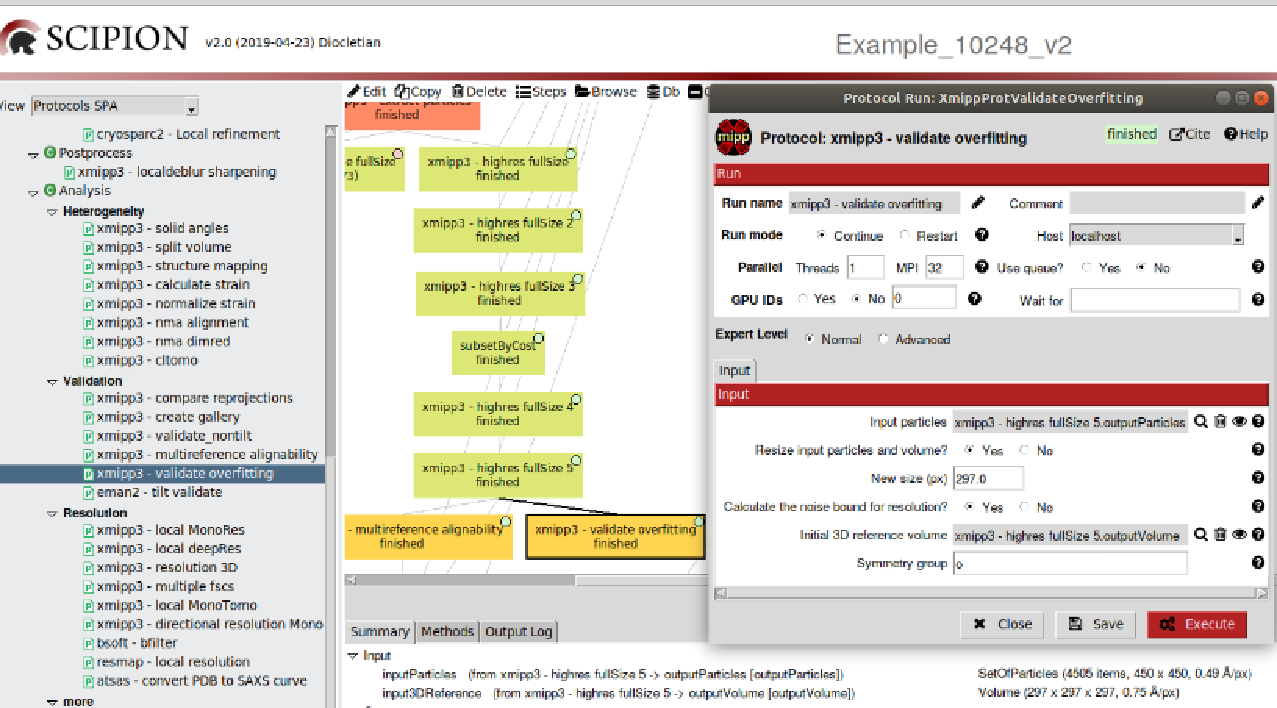
\includegraphics[width=0.95\textwidth]
  {{images/validate_overfitting.pdf}}
  \caption{Filling in the form of the protocol \scommand{xmipp3-validate overfitting}.}
  \label{fig:validate_overfitting}
  \end{figure}

The output values of particle alignment, precision and accuracy, generated by \scommand{xmipp3-multireference alignability} (press \scommand{Analyze Results} to check table columns \ttt{\_xmipp\_scoreAlignabilityAccuracy} and \ttt{\_xmipp\_scoreAlignabilityPrecission}) allow us to discard particles with worse alignment. In this case, 1,020 particles (22.6\% of the total input) are rejected. In order to improve the refined map resolution, the remaining 3,485 particles will be used to perform the sixth local refinement iteration with $Xmipp$ \ttt{highres} algorithm. The protocol params will remain unchanged compared with the fifth iteration.

\begin{figure}[H]
  \centering
  \captionsetup{width=.8\linewidth} 
  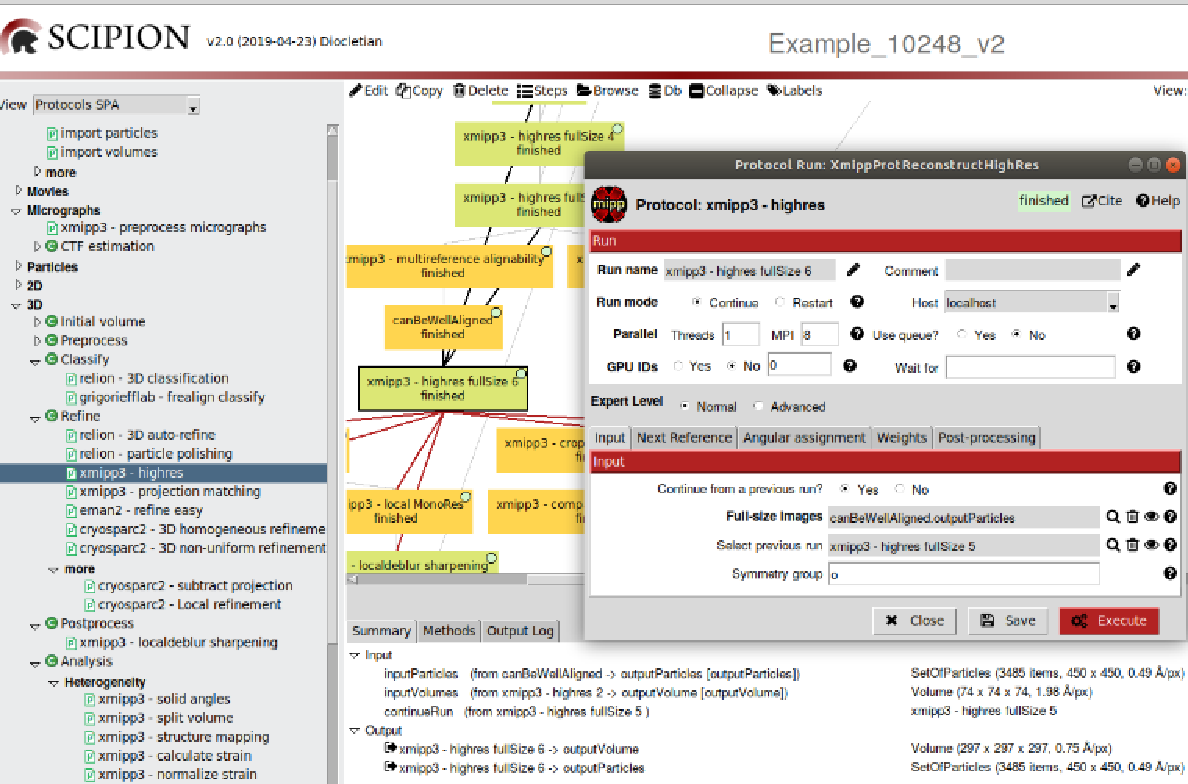
\includegraphics[width=0.95\textwidth]
  {{images/highres_fullsize6.pdf}}
  \caption{$Xmipp$ \ttt{highres} map local refinement (Iteration 6).}
  \label{fig:highres_fullsize6}
  \end{figure}

The sampling of the output map is the same than in the previous iteration, despite the selection of best aligned particles. We have thus achieved convergence and we can compute the global or local resolution. The local resolution can be calculated with the protocol \scommand{xmipp3-local MonoRes} \citep{vilas2018monores}. To have an overview of protocol and function of \ttt{MonoRes} see our \scipion tutorial in Model Building (download from \url{https://github.com/I2PC/scipion/wiki/tutorials/tutorial_model_building_basic.pdf}).                   
